% To je predloga za poročila o domačih nalogah pri predmetih, katerih
% nosilec je Blaž Zupan. Seveda lahko tudi dodaš kakšen nov, zanimiv
% in uporaben element, ki ga v tej predlogi (še) ni. Več o LaTeX-u izveš na
% spletu, na primer na http://tobi.oetiker.ch/lshort/lshort.pdf.
%
% To predlogo lahko spremeniš v PDF dokument s pomočjo programa
% pdflatex, ki je del standardne instalacije LaTeX programov.

\documentclass[a4paper,11pt]{article}
\usepackage{a4wide}
\usepackage{fullpage}
\usepackage[utf8x]{inputenc}
\usepackage[slovene]{babel}
\selectlanguage{slovene}
\usepackage[toc,page]{appendix}
\usepackage[pdftex]{graphicx} % za slike
\usepackage{setspace}
\usepackage{color}
\definecolor{light-gray}{gray}{0.95}
\usepackage{listings} % za vključevanje kode
\usepackage{hyperref}
\renewcommand{\baselinestretch}{1.2} % za boljšo berljivost večji razmak
\renewcommand{\appendixpagename}{Priloge}

\lstset{ % nastavitve za izpis kode, sem lahko tudi kaj dodaš/spremeniš
language=Python,
basicstyle=\footnotesize,
basicstyle=\ttfamily\footnotesize\setstretch{1},
backgroundcolor=\color{light-gray},
}

\title{Logistična regresija}
\author{Tilen Venko (63140280)}
\date{\today}

\begin{document}

\maketitle

\section{Uvod}

Naša naloga je bila izračunat verjetnost za posamezen primer, cenilno funkcijo in gradient cenilne funkcije. Nato preveriti vpliv lambde na rezultate, implementirati prečno preverjanje in mero napovedne točnosti. Za konec pa ustvariti dve skupini slik in jih pskusiti ločiti med sabo.

\section{Podatki}

Za slike sem si izbral skupino avtov in skupino čolnov. V orodju Orange sem slike s pomočjo ImageNet pretvoril v značilke in jih shranil kot images.csv.

\section{Metode}

Mero napovedne točnosti sem razvil v funkciji \textit{CA(real, predictions)}. Ki sprejme naše napovedi in pa testne podatke iz prečne validacije. Točnost preverjam s metodo RMSE.

\section{Rezultati}

\begin{figure}[htbp]
\begin{center}
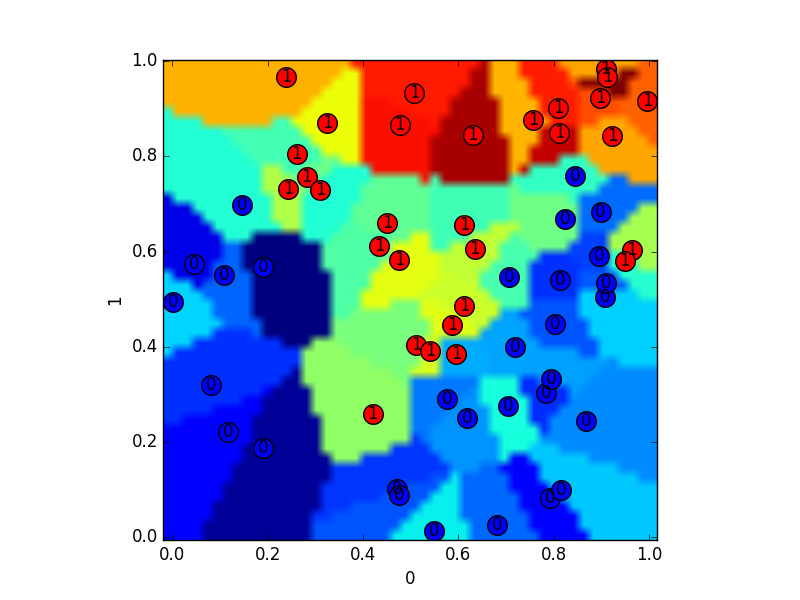
\includegraphics[scale=0.6]{lambda1.png}
\caption{Izris za lambda=0.1.}
\label{slika1}
\end{center}
\end{figure}

\begin{figure}[htbp]
\begin{center}
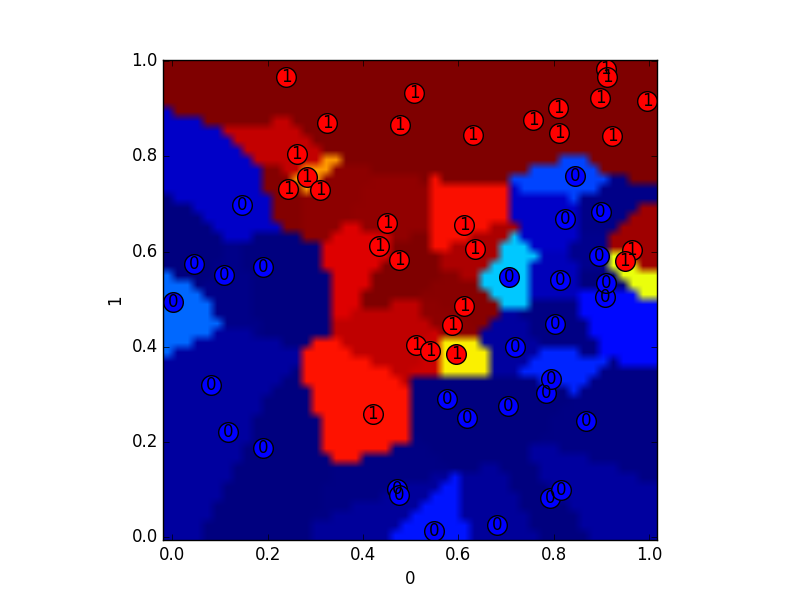
\includegraphics[scale=0.6]{lambda0001.png}
\caption{Izris za lambda=0.0001.}
\label{slika1}
\end{center}
\end{figure}

\begin{figure}[htbp]
\begin{center}
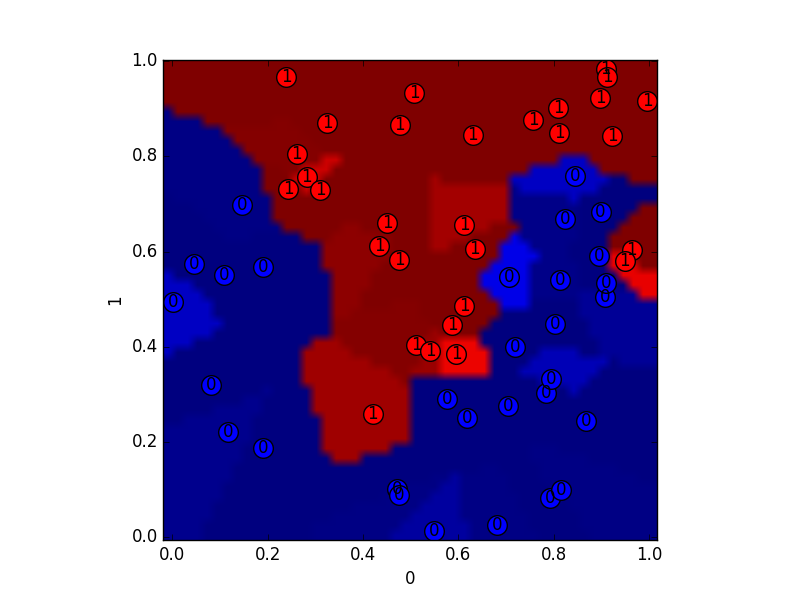
\includegraphics[scale=0.6]{lambda00001.png}
\caption{Izris za lambda=0.00001.}
\label{slika1}
\end{center}
\end{figure}

Pri lambdi 0.1 so skupine zelo razdrobljene in tezko bi karkoli napovedali iy tak[nega modela, pri lambdi 0.00001 nismo modela nič, kaj popravili od prvotnega modela brez regularizacije. Zato se mi zdi, da je najboljši model za lambda 0.0001, saj se lepo vidi za katere točke ne moramo biti povsem prepričani v katero kategorijo spadajo in za katere smo lahko precej prepričani, da spadajo v to kategorijo.\\
3. in 4. točke mi ni uspelo rešiti v ceoti.

\section{Izjava o izdelavi domače naloge}
Domačo nalogo in pripadajoče programe sem izdelal sam.

\end{document}
